\documentclass{article}

\usepackage{kotex}
\usepackage{graphicx}
\usepackage[affil-it]{authblk}
\usepackage{mathtools}
\usepackage{amssymb}
\usepackage{amsthm}
\usepackage{geometry}
\usepackage{fancyhdr}
\usepackage{braket}
\usepackage{cite}
\usepackage{cancel}
\usepackage{subcaption}
\usepackage{enumitem}
\usepackage{color}
\usepackage{booktabs}
\usepackage{chemformula}
\usepackage{physics}
\usepackage{hyperref}

\newcommand{\vp}{\varphi}
\newcommand{\ve}{\varepsilon}

\newtheorem{theorem}{Theorem}
\newtheorem{definition}[theorem]{Definition}
\newtheorem{example}[theorem]{Example}
\newtheorem{lemma}[theorem]{Lemma}
\newtheorem{axiom}[theorem]{Axiom}
\newtheorem{remark}[theorem]{Remark}
\newtheorem{problem}[theorem]{Problem}
\newtheorem{exercise}[theorem]{Exercise}

\counterwithin{equation}{section}
\counterwithin{theorem}{section}


\geometry{a4paper,left=2cm,right=2cm,top=2.4cm,bottom=2.4cm}

\linespread{1.3}

\title{\textsf{Free Energy and Chemical Thermodynamics}}
\author[1]{Written by Eun Taek Kang\thanks{email: etkang03@gmail.com}}
\affil[1]{Department of Physics, Sogang University, Seoul 04107, Korea}

\date{Summer 2025, Sogang University}

\begin{document}

\pagestyle{fancy}
    %... then configure it.
    \fancyhf{}
    % Set the header and footer for Even
    % pages but omit the zone (L, C or R)
    \fancyhead[R]{\textsf{Prof.\ Hyeonjun Baek}}
    \fancyhead[L]{\textsc{Thermal Physics}}
    \fancyfoot[C]{\thepage}
    \fancyfoot[L]{\textbf{Sogang University}}
    \fancyfoot[R]{\textit{Department of Physics}}

\maketitle

\begin{abstract}
    백현준 교수님께서 2025년 1학기에 진행하는 열역학 기말고사 대비를 위해 만든 Note입니다. 이 문서는 Daniel V. Schroeder 저 An Introduction to Thermal Physics의 Chapter 5. Free Energy and Chemical Thermodynamics를 다루고 있습니다.
\end{abstract}

\newpage

\section{Free energy as available work}

\textbf{Thermodynamics Potentials}

우리는 어떠한 계의 에너지를 $U$로 표현했다. 이제, 3가지의 새로운 열역학 퍼텐셜들을 정의할 것이다.
\begin{equation}
    \boxed{H \equiv U + PV} \quad \boxed{F \equiv U - TS} \quad \boxed{G \equiv U - TS + PV}
\end{equation}
$H$는 엔탈피(enthalpy), $F$는 헬름홀츠 자유에너지(Helmholtz free energy), $G$는 깁스 자유에너지(Gibbs free energy)라고 한다. 

\begin{figure}[h]
\centering
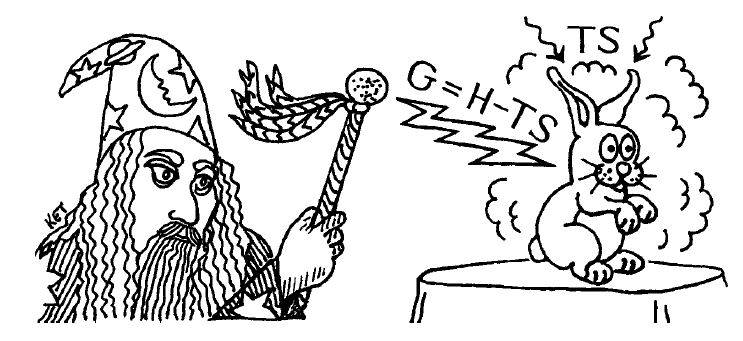
\includegraphics[width=0.6\linewidth]{images/fig1_1.png}
\end{figure}

토끼를 만드는 상상도에서 비유해보자. 탁자 위에 토끼를 만드는데 필요한 에너지는 엔탈피 $H=U+PV$이다. 그 중에 열 때문에 $TS$정도는 자연적으로 유입이 가능함. 따라서 마법사가 필요한건 깁스 자유에너지 $G=H-TS$만큼이 필요한거다. \underline{법사가 $G$만큼만 걸어줘도 토끼가 만들어져요!}

\begin{figure}[h]
\centering
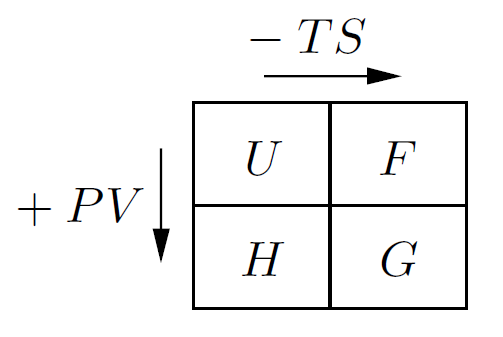
\includegraphics[width=0.4\linewidth]{images/fig1_2.png}
\end{figure}

\noindent
\textcolor{red}{따라서, 우리는 위의 diagram을 필히 외워두도록 하자. 헷갈릴 때 저 diagram을 이용하면 혼돈을 막을 수 있다.}

\begin{itemize}
    \item 온도 $T$가 일정할 때, $\Delta F = \Delta U - T\Delta S = Q + W - T\Delta S$이다. 
    
    $Q$는 가한 열, $W$는 계에 해준 일이다. 일반적으로 $Q \leq T\Delta S \ \Rightarrow \ \Delta F \leq W$이다. (엔트로피 안 생기면 등호 성립) 특히, $W$는 환경의 수축 및 팽창에 의한 일도 포함한다.

    \item 온도 $T$와 압력 $P$가 일정할 때, $\Delta G = \Delta U - T \Delta S + P \Delta V = Q + W - T \Delta S + P \Delta V$이다.
    
    이때, $W = -P\Delta V + W_{\text{other}}$이다. ($-P\Delta V$는 환경에 의한 일), 역시 $Q \leq T\Delta S$이므로, $\Delta G \leq W$이다!
\end{itemize}

특히나 깁스 자유에너지를 다음과 같이 계산하는 방법은 자주 쓰인다.
\begin{equation}
    \Delta G = \Delta H - T \Delta S
\end{equation}

\newpage

\noindent
\textbf{Electrolysis, Fuel cells, and Batteries} \textcolor{blue}{(Free energy example!)}

\vspace{1mm}
물의 전기 분해부터 살펴보자. $\ch{H2 O} \rightarrow  \ch{H2} + \dfrac{1}{2} \ch{O2}$인건 명백하다.

\begin{figure}[h]
\centering
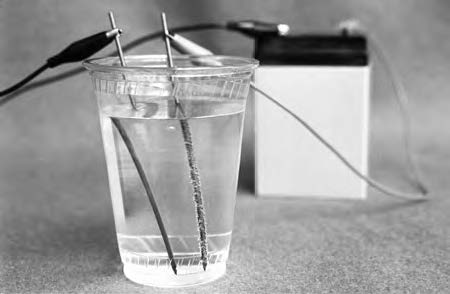
\includegraphics[width=0.35\linewidth]{images/fig1_3.jpeg}
\end{figure}

여기서, 깁스 자유 에너지는 다음과 같다.
\begin{equation}
    \Delta G = \Delta H - T \Delta S = \Delta U + P\Delta V - T \Delta S
\end{equation}
1몰의 물에서 일어나는 에너지 출입의 모식도는 이렇다.

\begin{figure}[h]
\centering
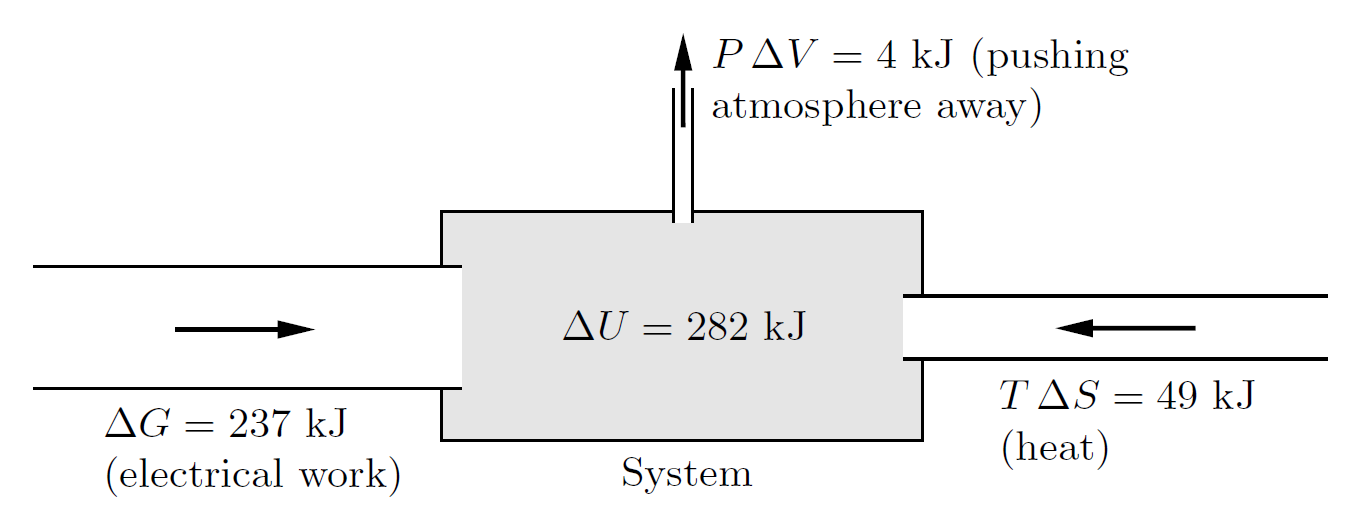
\includegraphics[width=0.65\linewidth]{images/fig1_4.png}
\end{figure}

계에 해준 일과 열에 의한 유입 에너지를 계산해보자.\footnote{131, 205, 70같은 숫자는 화학책 표에서 찾는다. 크게 신경쓸 값은 아님.}
\begin{equation}
    P \Delta V = (\Delta n) R T = (1 + 1/2) \cdot (8.31) \cdot (293) \approx 4 \text{kJ}
\end{equation}
\begin{equation}
    T \Delta S = \left[ \left( 131 + \frac{1}{2} \cdot 205 \right) -70 \right] \cdot (293) \approx 49 \text{kJ}   
\end{equation}
다음은 수소 연료를 알아보자. 

\begin{figure}[h]
\centering
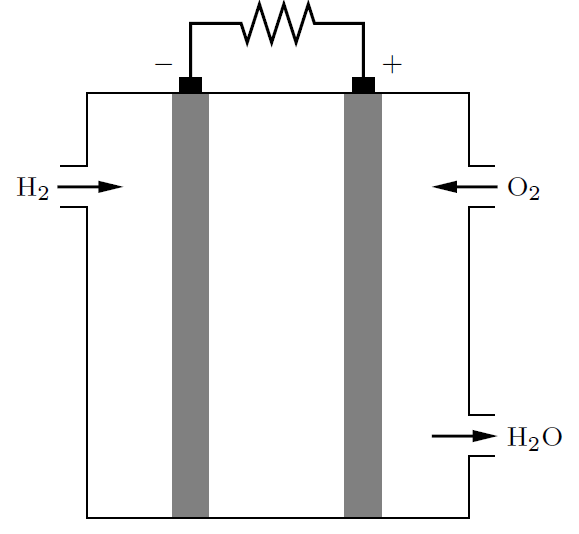
\includegraphics[width=0.3\linewidth]{images/fig1_5.png}
\end{figure}

이 과정에선 반응식이 반대로 $\ch{H2 O} \leftarrow  \ch{H2} + \dfrac{1}{2} \ch{O2}$이다. 또한, 위의 모식도의 모든 화살표 방향이 반대가 되고, $\Delta U = -282$ kJ가 된다. 또한, 이상적인 연료의 효율성을 계산하면 다음과 같다.
\begin{equation}
    \frac{|\Delta G|}{|\Delta U|} = \frac{237}{286} \approx 83 \%
\end{equation}

\newpage

마지막으로, 배터리를 알아볼 것이다. 배터리는 다음과 같은 모식도를 가진다.

\begin{figure}[h]
\centering
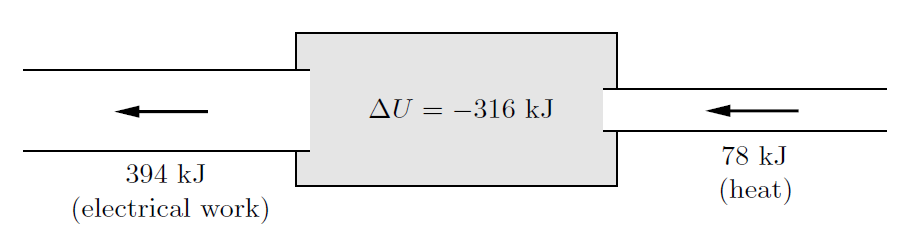
\includegraphics[width=0.6\linewidth]{images/fig1_6.png}
\end{figure}

\noindent
신기한 점은, 배터리는 $\Delta U \approx \Delta H$이고, $\Delta F \approx \Delta G$이다. 배터리의 반응식은 다음과 같다.
\begin{equation*}
    \ch{Pb} + \ch{Pb O2} + \ch{4 H+} + \ch{2 SO4 ^{2-}} \rightarrow \ch{2 Pb SO4} + \ch{2 H2 O}
\end{equation*}
이는 다음의 3단계로 반응이 일어난다.
\begin{align*}
    \text{in solution} &: \ch{2 SO4 ^{2-}} + \ch{2 H+} \rightarrow \ch{2 HSO4-}\\
    \text{at $-$ electrode} &: \ch{Pb}  + \ch{HSO4-} \rightarrow \ch{PbSO4} + \ch{H+} + \ch{2 e-}\\
    \text{at $+$ electrode} &: \ch{PbO2} + \ch{HSO4- } + \ch{3 H+}  + \ch{2 e-} \rightarrow \ch{Pb SO4} + \ch{2 H2O}
\end{align*}
또한, 이때 전자 1개 당 해준 전기적 일은 다음과 같다.
\begin{equation}
    \frac{394 \text{kJ}}{2 \cdot 6.02 \times 10^{23}} = 3.27 \times 10^{-19} \text{J} = 2.04 \text{eV}
\end{equation}

\noindent
\textbf{Thermodynamic identities}

앞서, 우린 아주 중요한 에너지의 전미분을 배웠다.
\begin{equation}
    \boxed{dU = Tds - PdV + \mu dN}
\end{equation}
헬름홀츠 자유에너지 $F = U - TS$에 적용해보자.
\begin{equation}
    dF = dU - Tds - SdT = (Tds - PdV + \mu dN) - Tds - SdT = \boxed{-PdV + \mu dN - SdT}
\end{equation}
따라서, 우리는 헬름홀츠 자유에너지는 $T, V, N$에 대한 함수 $F(T,V,N)$으로 쓸 수 있고, 다음 identities가 성립한다.
\begin{equation}
    \boxed{P = -\left( \frac{\partial E}{\partial V} \right)_{T, N}} \quad \boxed{\mu = \left( \frac{\partial E}{\partial N} \right)_{T, V}} \quad \boxed{S = -\left( \frac{\partial E}{\partial T} \right)_{V, N}}
\end{equation}
이제, 다음 3가지 중요한 전미분을 기억하자.
\begin{align}
    \boxed{dS = \frac{1}{T} dU + \frac{P}{T} dV - \frac{\mu}{T} dN} \quad \boxed{dU = T\,dS - P\,dV + \mu\,dN} \quad \boxed{dF = -S\,dT - P\,dV + \mu\,dN}
\end{align}
이로부터, 중요한 편미분 identity들을 얻을 수 있다. 진짜 개중요하니 알아두자. 모르면 쉽지 않다.

\begin{table}[h]
\centering
\begin{tabular}{@{}cccc@{}}
\toprule
 & $S(U,V,N)$ & $U(S,V,N)$ & $F(T,V,N)$ \\ \midrule
$T$ &
  $\dfrac{1}{T} = \left( \dfrac{\partial S}{\partial U} \right)_{V, N}$ &
  $T = \left( \dfrac{\partial U}{\partial S} \right)_{V, N}$ &
  $T \text{ is given.}$ \\
$P$ &
  $\dfrac{P}{T} = \left( \dfrac{\partial S}{\partial V} \right)_{U, N}$ &
  $P = - \left( \dfrac{\partial U}{\partial V} \right)_{S, N}$ &
  $P = - \left( \dfrac{\partial F}{\partial V} \right)_{T, N}$ \\
$\mu$ &
  $- \dfrac{\mu}{T} = \left( \dfrac{\partial S}{\partial N} \right)_{U, V}$ &
  $\mu = \left( \dfrac{\partial U}{\partial N} \right)_{S, V}$ &
  $\mu = \left( \dfrac{\partial F}{\partial N} \right)_{T, V}$ \\ \bottomrule
\end{tabular}
\caption{Thermodynamic Potentials의 identities}
\label{tab:1}
\end{table}

\newpage

깁스 자유 에너지에 대한 identities도 뽑을 수 있는데, 먼저 깁스 자유 에너지의 전미분을 구해보자.
\begin{align}
    \boxed{G = U - TS + PV } \quad \rightarrow \quad dG &= dU - TdS- SdT + PdV + VdP\\ \nonumber
    &= (\cancel{TdS} - \cancel{PdV} + \mu dN) - \cancel{TdS} - SdT + \cancel{PdV} + VdP\\
    &\Rightarrow \boxed{ dG = -SdT + VdP + \mu dN}
\end{align}
따라서, $G$를 변수들을 통해 나타내주면 $G = G(S,P,N)$이고, 편미분 identities는 다음과 같다.
\begin{equation} \label{eq:1-14}
    \boxed{S = - \left( \frac{\partial G}{\partial T} \right)_{P,N}} \quad \boxed{V = \left( \frac{\partial G}{\partial P} \right)_{T,N}} \quad \boxed{\mu = \left( \frac{\partial G}{\partial N} \right)_{T,P}}
\end{equation}
이것들은 전부 \underline{system이 단일 종류의 입자라는 가정}에서나 맞고, 만약 다종류 입자 system이라면 화학 퍼텐셜 $\mu$들이 달라진다. $\mu d N$이 그들의 전체 합으로 대체되어야 한다. 따라서, 예를 들어 입자가 $k$개면 다음과 같다.
\begin{equation}
    \mu_1 = \left( \frac{\partial G}{\partial N_1} \right)_{T, P, N_2, N_3, \cdots, N_k} \quad \mu_2 = \left( \frac{\partial G}{\partial N_1} \right)_{T, P, N_1, N_3, \cdots, N_k}
\end{equation}

\section{Free Energy as a force toward equilibrium}

고립계에선 보통 엔트로피는 증가한다. 근데, 비고립계에선 어떨까??

\begin{figure}[h]
\centering
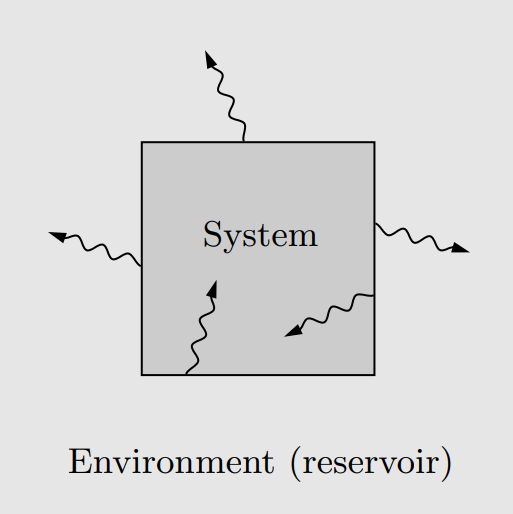
\includegraphics[width=0.25\linewidth]{images/fig2_1.png}
\end{figure}

이렇게 주변이랑 에너지 교환은 가능한 고립계를 생각해보자.\footnote{외부 환경이랑 에너지 교환마저 안되면 이걸 닫힌계(closed system)라고 한다.} 엔트로피는 크게 표현해주면 다음과 같다.
\begin{equation}
    dS_{\text{total}} = dS_s + dS_R 
\end{equation}
이때, \textcolor{blue}{$T,V,N$은 고정된 상태이다.} 그러면 다음 식에 의하여 \underline{에너지 $U$만 변할 수 있다.}
\begin{equation}
    dS = \frac{1}{T}dU + \frac{P}{T}dV - \frac{\mu}{T} dN
\end{equation}
엔트로피는 에너지에 의존하는 변수이므로, $S(U)$ 형태로 분석해보자.
\begin{align}
    S_{\text{tot}} &= S_s(U_s) + S_R (U_{\text{tot}} - U_s)\\ \nonumber
    &\approx S_s(U_s) + S_R (U_{\text{tot}}) - U_s \left( \frac{\partial S_R}{\partial U_R} \right)_{V,N} \quad (U_s \ll U_\text{tot}, \ \text{Taylor Expansion})\\
    &= S_R (U_{\text{tot}}) - \frac{1}{T_s} \cdot U_s + S_s (U_s) \qquad \qquad  \left[ \left( \frac{\partial S_R}{\partial U_R} \right)_{V,N} = \frac{1}{T_R} = \frac{1}{T_S} \right]
\end{align}
따라서 $V,N,T$가 일정할 때, $S$가 증가할 수록, $F$는 감소한다. 여기서 $\Delta F \leq W$에 의하면, 따로 계에 일을 가하지 않으면 $F$는 감소한다.

\newpage

만약, $T,P,N$이 고정되어 있다면 어떨까? 쉽게 말해 계의 부피도 변할 수 있단 가정을 해보자는 것이다. 수식적으론, $S$를 결정하는데 $U, V$가 관여한다는 것이다.\footnote{교과서엔 자세하게 없는 내용이다.}
\begin{align}
    S_{\text{tot}} &= S_s(U_s , V_s) + S_R (U_{\text{tot}} - U_s , V_{\text{tot}} - V_s)\\ \nonumber
    &\approx S_R(U_{\text{tot}}, V_{\text{tot}}) - \left( \frac{\partial S_R}{\partial U_R} \right)_{V,N} U_s - \left( \frac{\partial S_R}{\partial V_R} \right)_{U,N} V_s + S_s(U_s, V_s)\\
    &= S_R(U_{\text{tot}}, V_{\text{tot}}) - \frac{U_s}{T_s} - \frac{P_s}{T_s} \cdot V_s + S_s(V_s, U_s) \quad \left[ \left( \frac{\partial S_R}{\partial V_R} \right)_{U,N} = \frac{P_R}{T_R} = \frac{P_S}{T_S} \right]
\end{align}
따라서, $T,P,N$이 일정할 때, $S$가 증가할 수록 $G$는 감소한다. 이 역시 $\Delta F \leq W$에 의한 결과이다. 그러고 나서 $F$와 $G$의 정의를 다시 보자.
\begin{equation}
    F \equiv U - TS \qquad G \equiv U - TS + PV
\end{equation}
이를 종합하면, \textbf{고온에선 $S$가, 저온에선 $U$가} 에너지의 경향성을 지배한다고 할 수 있다.

\vspace{3mm}\noindent
\textbf{Minimum of $F=U-TS$}

\begin{center}
    \fbox{헬름홀츠 자유에너지($F$)는 equilibrium(평형점)에서 최소이다.}    
\end{center}
이 명제에 의하여 직관적으로 다음을 얻을 수 있다.
\begin{equation}
    \mu = \left( \frac{\partial F}{\partial N} \right)_{T,V}, \qquad P = - \left( \frac{\partial F}{\partial V} \right)_{T,N}
\end{equation}
다음과 같이 두 system이 마주보고 겹쳐 있다 하자.

\begin{figure}[h]
    \centering
    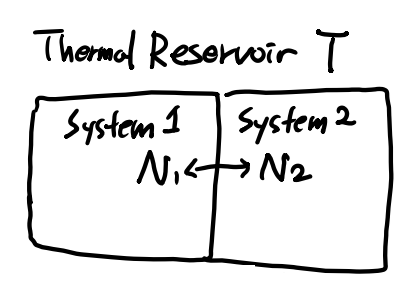
\includegraphics[width=0.3\linewidth]{images/fig2_2.png}
\end{figure}

\noindent
처음으로, $V_1, V_2$는 고정이고, $N_1 + N_2 = N_{\text{tot}}$라고 하자. 평형점에선 헬름홀츠 자유에너지의 합 $F_1 + F_2$는 최소다. 따라서
\begin{equation}
    \frac{\partial (F_1 + F_2)}{\partial N_1} = 0 = \frac{\partial F_1}{\partial N_1} + \frac{\partial F_2}{\partial N_2} = \frac{\partial F}{\partial N_1} - \frac{\partial F_2}{\partial N_2} \quad \Rightarrow \quad \frac{\partial F_1}{\partial N_1} = \frac{\partial F_2}{\partial N_2} \ \ (\mu_1 = \mu_2)
\end{equation}
만약, $N_1, N_2$가 고정되어 있고, $V_1 + V_2 = V$라고 한다면, 다음이 성립한다.
\begin{equation}
    \frac{\partial F_1}{\partial V_1} = \frac{\partial F_2}{\partial V_2} \ \ (P_1 = P_2)
\end{equation}

\newpage

\noindent
\textbf{Extensive and Intensive quantities}

\begin{figure}[h]
    \centering
    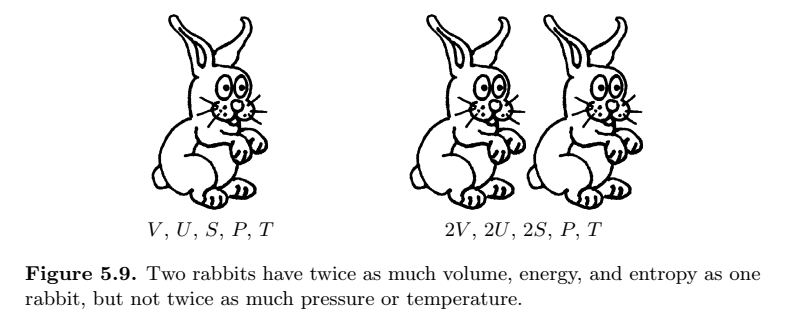
\includegraphics[width=0.7\linewidth]{images/fig2_3.png}
\end{figure}

열역학에서 변수들이 상당히 많이 나왔다. 이들은 다음과 같다.
\begin{equation*}
    U, \ V, \ N, \ S, \ T, \ P, \ \mu, \ H, \ F, \ G, \ m, \ \rho, \ C, \ c
\end{equation*}
\cancel{진짜 드럽게도 많다..} 여하튼, 이것들을 크게 2가지 종류의 변수로 구분할 수 있다. \textbf{크기변수}(extensive)는 계를 2배로 하면 함께 2배가 되는 물리량이고, \textbf{세기변수}(Intensive)는 함께 2배가 되지 않는 물리량이다. 위의 토끼 그림을 보면 된다. 따라서 분류하면 다음과 같다.
\begin{align*}
    \text{Extensive: }&V, \ N, \ S, \ U, \ H, \ F, \ G, \ m,\ C \\
    \text{Intensive: }&T, \ P, \ \mu, \ \rho, \ c
\end{align*}
Thermodynamic Identity나 Free Energy를 보면 다음과 같다.
\begin{align}
    dU &= TdS - PdV + \mu dN &(U, S, V, N \text{ Ex. } / \ T, P, \mu \text{ In.})\\
    F &= U - TS &(U, S \text{ Ex. } / \ T \text{ In.})\\
    G &= U + PV - TS &(U, S, V \text{ Ex. } / \ T, P \text{ In.})
\end{align}

\noindent
\textbf{Gibbs free energy and Chemical Potential}

깁스 자유 에너지의 전미분과 그로부터 얻는 관계는 다음과 같다.
\begin{align}
    dG = - SdT + VdP + \mu dN  \quad &\Rightarrow \quad G=G(T,P,N) = N \cdot Q(T,P)\\ \nonumber
    &\Rightarrow \quad \left( \frac{\partial G}{\partial N} \right)_{T,P} = Q(T,P) \ \ \text{by }(\ref{eq:1-14})\\
    &\Rightarrow \quad \mu = Q (T,P) \ \ \Rightarrow \ \ G = \mu N \label{eq:2-15}
\end{align}
이 식은 계에 입자를 1개 추가할 때마다 깁스 자유에너지가 $\mu$씩 증가함을 나타낸다. 이제, 다양한 종류의 입자들을 포함하면 (\ref{eq:2-15})를 다음과 같이 일반화할 수 있다.
\begin{equation}
    G = N_1 \mu_1 + N_2 \mu_2 + \cdots = \sum_i N_i \mu_i
\end{equation}
이제, $T,N$이 고정된 상태에서 (\ref{eq:2-15})를 결합시키면, 다음이 성립한다.
\begin{equation}
    \left( \frac{\partial \mu}{\partial P} \right)_{T,N} = \frac{\partial }{\partial P} \left( \frac{G}{N} \right)_{T,N} = \frac{1}{N} \left( \frac{\partial G}{\partial P} \right)_{T,N} = \frac{1}{N} \cdot V = \frac{kT}{P} \quad \text{(In ideal gas)}
\end{equation}
이제 양쪽을 $P^\circ$부터 $P$까지 적분해주면 다음과 같다. ($P^\circ$는 보통 1 atm으로 둔다.)
\begin{equation}
    \mu(T,P) = \mu(T, P^\circ) + kT \ln \left( \frac{P}{P^\circ} \right)
\end{equation}
이 식은, 압력이나 밀도가 변할 때, $\mu$는 어떻게 변하는지 보여준다.

\newpage

\section{Phase Transformations od Pure Substances}

상변화(phase transformation)란, 물질의 환경이 아주 미세하게 변화함에도 불구하고 그 성질이 불연속적으로 바뀌는 현상을 말한다. 우리는 이걸 깁스 자유에너지를 통해 이해해볼 것이다.

\begin{figure}[h]
    \centering
    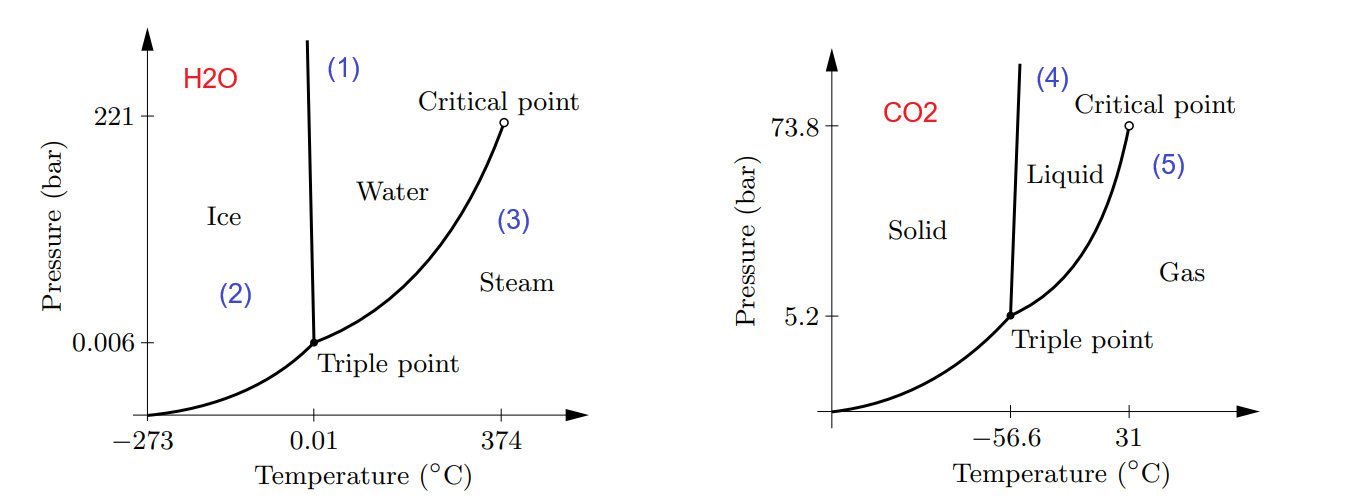
\includegraphics[width=0.95\linewidth]{images/fig3_1.png}
\end{figure}

\begin{enumerate}
    \item[(1)] 선 위에서는 두 개의 서로 다른 상이 공존할 수 있다.
    \item[(2)] 얼음은 특이하게도 압력을 높이면 녹는점이 낮아진다. 이는 얼음이 물보다 밀도가 작아서 그렇다. (곧 확인)
    \item[(3)] 액체-기체 경계선은 항상 양의 기울기를 가진다. 
    \item[(4)] 대부분의 물질은 압력이 증가하면 녹는점도 증가한다.
    \item[(5)] 유체에선 액체가 기체로 변할 때 불연속적인 변화가 없다.
\end{enumerate}

\noindent
\textbf{Helium's exotic phase transformation among all elements}

헬륨은 상 행동이 아주 특이하게 일어난다. 상변화 그림을 보자.

\begin{figure}[h]
    \centering
    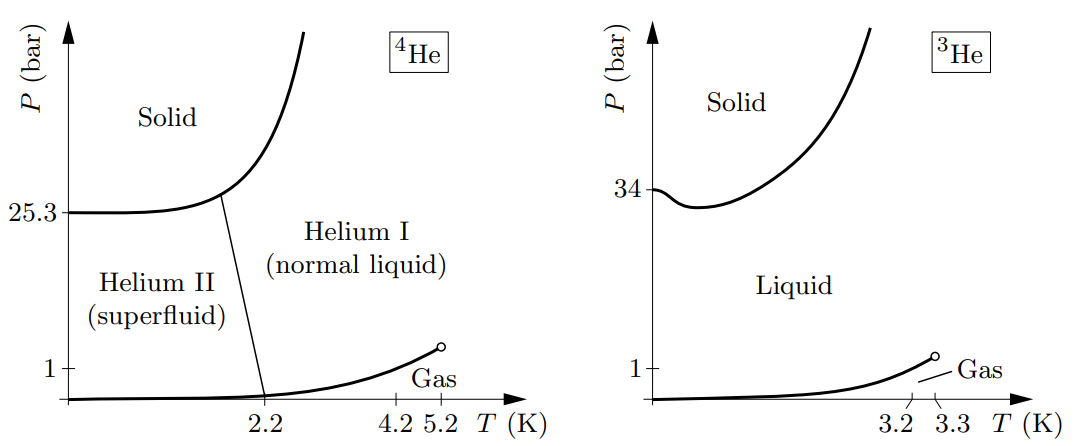
\includegraphics[width=0.78\linewidth]{images/fig3_2.png}
\end{figure}

\begin{itemize}
    \item 헬륨은 유일하게 0K(절대온도)에서도 액체 상태로 존재하는 원소이다.
    \item 특히, 헬륨 II같이 초유체 상태는 매우 특별한 성질들을 가지며, 그 중에는 무점성(zero viscosity)과 매우 높은 열전도율이 있다. (실험에서 액화 헬륨을 자주 쓰는 이유, 다만 아주 비싸다.)
\end{itemize}

\newpage

상변화를 일으키는데는 온도, 압력뿐 아니라 조성, 자기장 세기들도 영향을 미친다. 

\begin{figure}[h]
    \centering
    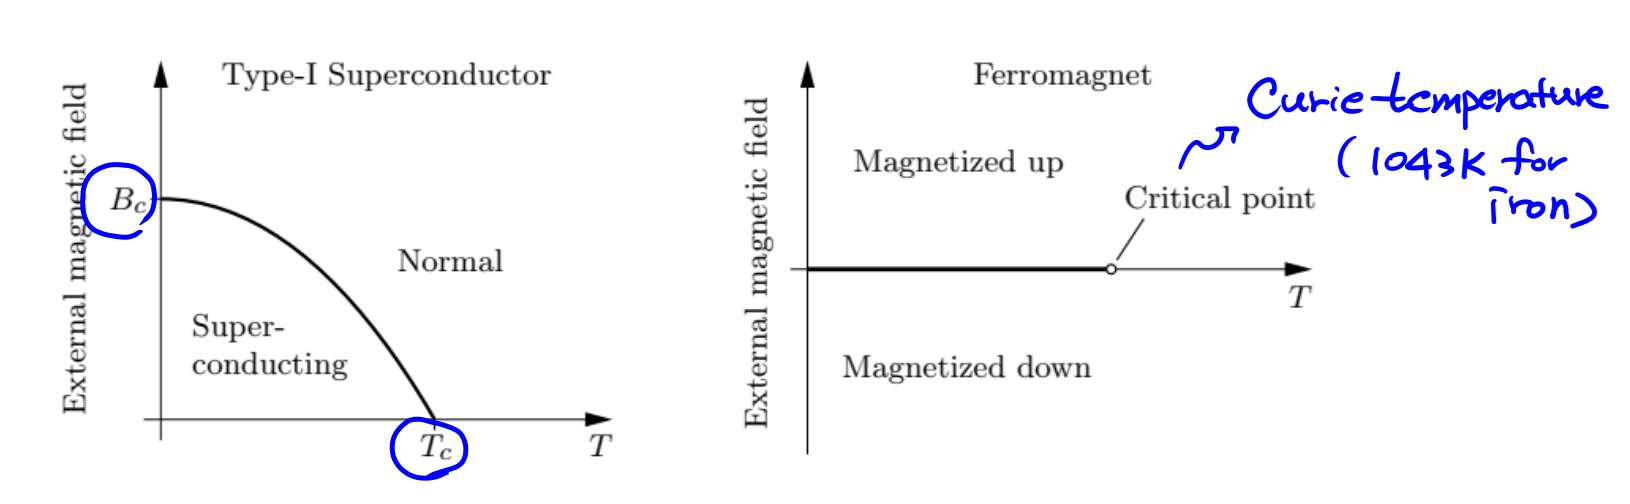
\includegraphics[width=0.9\linewidth]{images/fig3_3.png}
\end{figure}

\noindent
\textbf{Diamonds and Graphite}

(\ref{eq:1-14})에서 봤던 $V$에 대한 identity를 떠올리자.

\begin{figure}[h]
    \centering
    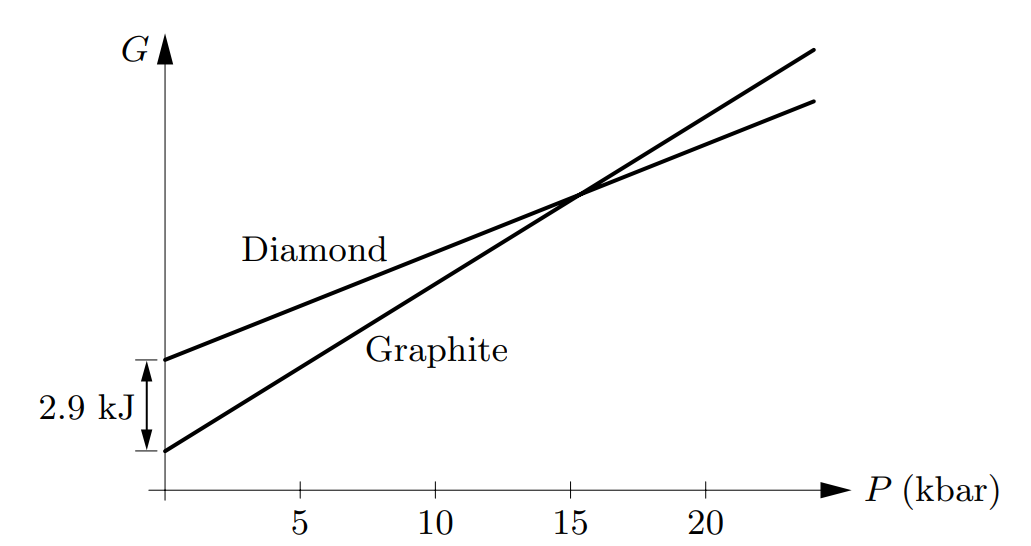
\includegraphics[width=0.6\linewidth]{images/fig3_4.png}
\end{figure}

\begin{itemize}
    \item 보통 상온, 상압에선 깁스 자유 에너지가 흑연이 다이아몬드보다 낮다. ($G_{\text{dia}} > G_{\text{gra}}$)
    \item 상압에선 흑연이 다이아몬드보다 안정된 상이다. 고로, 다이아몬드는 흑연으로 변하려 하지만, 상온에선 매우 느리게 일어난다.
    \item $V_{\text{gra}} > V_\text{dia}$에서, 그림의 $G-P$ 그래프 기울기는 흑연이 더 크다.
    \item 다만, 15 kbar 이상에선 흑연이 다이아몬드로 변한다.
\end{itemize}

\newpage

\noindent
\textbf{The Clausius-Calpeyron relation}

일단 다음과 같은 관계식을 기억해보자.
\begin{equation}
    \left( \frac{\partial G}{\partial T} \right)_{P,N} = -S, \quad \left( \frac{\partial S}{\partial P} \right)_{T,N} = V
\end{equation}
$P-T$ 그래프 그릴 때, 경계선의 기울기 양상은 두 상의 $S,V$ 차이와 연관이 있다. 

\begin{figure}[h]
    \centering
    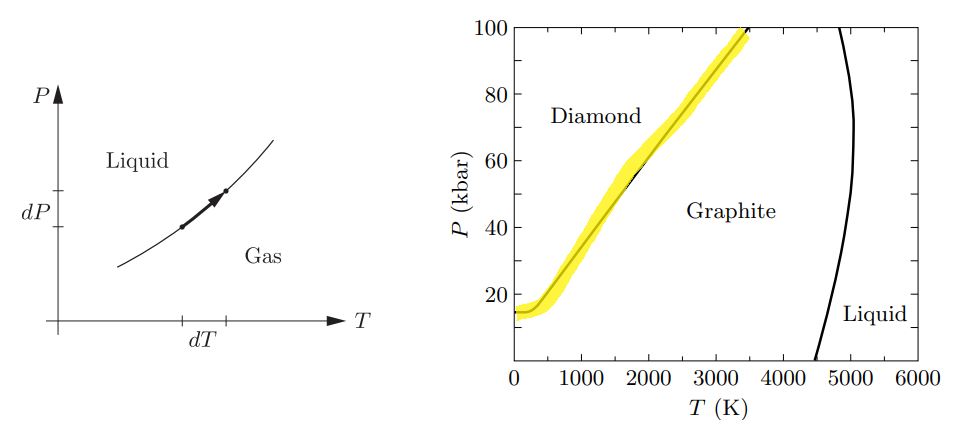
\includegraphics[width=0.8\linewidth]{images/fig3_5.png}
\end{figure}

기본적으로 상의 경계선에선, 두 상태의 깁스 자유 에너지가 같아야한다. ($dG_l = dG_g$) 다음 열역학적 identity를 다시 떠올리자.
\begin{equation}
    dG = -SdT + VdP
\end{equation} 
따라서, 다음이 성립한다.
\begin{equation}
    -S_{l} dT + V_l dP = -S_g dT  + V_g dP \ \ \Rightarrow \ \ \boxed{\frac{dP}{dT} = \frac{S_g - S_l}{V_g - V_l} = \frac{L}{\Delta V T}}
\end{equation}
여기서 $L$은 잠열이다. 우리는 박스 친 관계를 Clausius-Calpeyron relation이라고 한다. 실제로, 상온에서 1몰의 다이아몬드가 흑연이 될 때, 부피는 $1.9 \times 10^{-6}$m$^{3}$ 증가하고, 엔트로피는 3.4J/K 증가한다. 따라서,  상 경계의 기울기는 다음과 같다.
\begin{equation}
    \frac{dP}{dT} = \frac{\Delta S}{\Delta V} = \frac{3.4 \text{J/K}}{1.9 \times 10^{-6}\text{m}^3} = 18 \text{ bar/K}
\end{equation}

\noindent
\textbf{The Vander Waals model}

반데르 발스 방정식은 다음과 같다.
\begin{equation}\label{eq:3-5}
    \left( P + \frac{aN^2}{V^2} \right)(V-Nb) = NkT
\end{equation}
여기서, $a$는 분자의 양에 따른 비례상수, $b$는 분자가 이웃 분자와 닿아 있을 때, 분자 하나가 차지하는 최소한의 부피이다. 이 두 상수는 분자에 따라 다르다.

\begin{figure}[h]
    \centering
    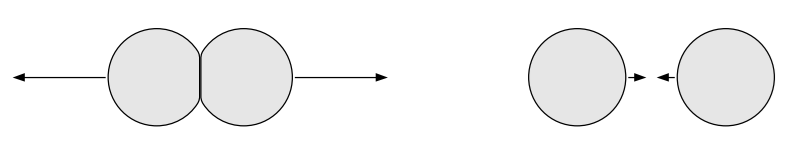
\includegraphics[width=0.7\linewidth]{images/fig3_6.png}
    \caption{두 분자가 너무 가까우면 밀어내고, 멀면 잡아 당긴다.}
\end{figure}

\newpage

Attraction potential energy는 $-aN^2/V$이고, 끌어당김에 의한 압력은 다음과 같다.
\begin{equation}
    P_{\text{att}} = - \left( \frac{\partial U}{\partial V} \right)_S = -\frac{d}{dV} \left(- \frac{aN^2}{V} \right) = - \frac{aN^2}{V^2}
\end{equation}
(\ref{eq:3-5})의 반데르발스 방정식을 그래프로 나타내면 다음과 같다. 그래프는 온도에 따라 달라진다.

\begin{figure}[h]
    \centering
    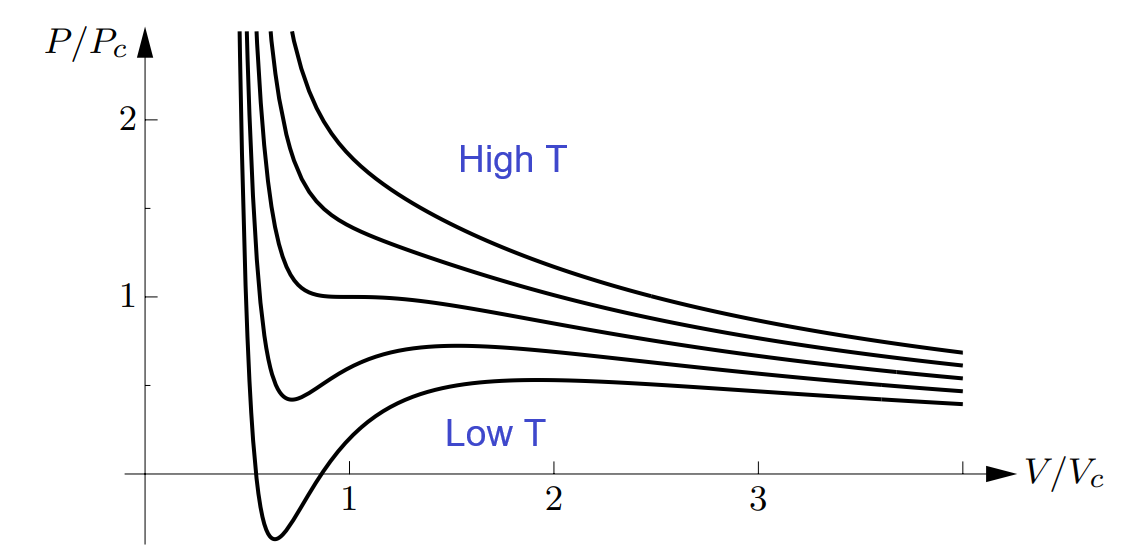
\includegraphics[width=0.55\linewidth]{images/fig3_7.png}
\end{figure}
$G$에 대한 열역학 항등식을 다시 떠올리자. ($dG = -SdT + VdP + \mu dN$) 만약 $N, V$가 고정이라면
\begin{equation}
    dG = VdP \quad \Rightarrow \quad \left( \frac{\partial G}{\partial V} \right)_{N,T} = V \left( \frac{\partial P}{\partial V} \right)_{N,T}
\end{equation}
반데르발스 방정식을 통해 나타낸 우변은 다음과 같다.
\begin{equation}
    \left( \frac{\partial P}{\partial V} \right)_{N,T} = -\frac{NkT}{(V-Nb)^2} + \frac{2aN^2}{V^3}
\end{equation}
이 결과를 통해 해석한 좌변은 이렇다.
\begin{align}
    \left( \frac{\partial G}{\partial V} \right)_{N,T} &= -\frac{NkTV}{(V-Nb)^2} + \frac{2aN^2}{V^2}\\
    &= -\frac{NkT(V-Nb)}{(V-Nb)^2} - \frac{NkT\cdot(Nb)}{(V-Nb)^2} + \frac{2aN^2}{V^2}\\
    &\Rightarrow  G = -NkT \ln (V-Nb) + \frac{NkT\cdot(Nb)}{(V-Nb)} - \frac{2aN^2}{V} + c(T,N)
\end{align}
여기서 $c(T,N)$은 양 변을 $V$에 대해 적분했기에 나오는 적분 상수이다.

\begin{figure}[h]
    \centering
    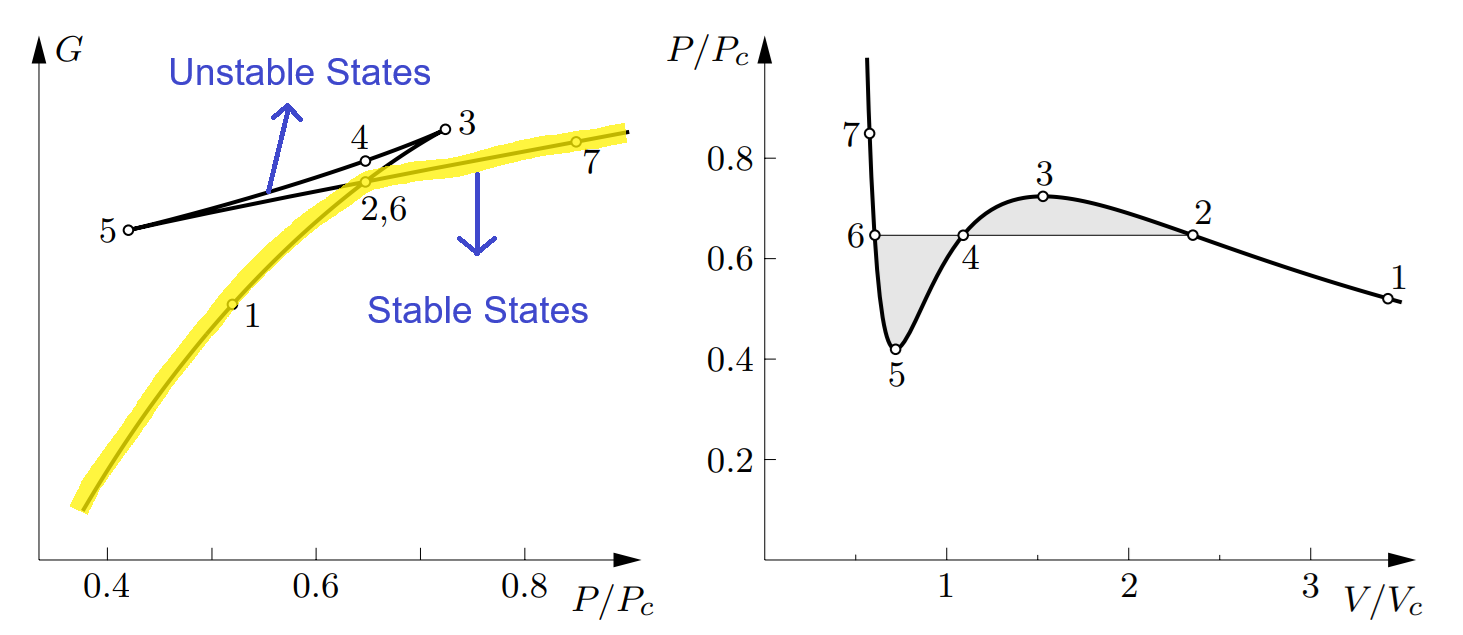
\includegraphics[width=0.75\linewidth]{images/fig3_8.png}
\end{figure}

$P-V$ 그래프에서 상변화 구간을 살펴보면, 압력이 점차 증가하면, 시스템은 점 2에서 점 6으로 곧바로 이동하며 부피가 갑자기 감소하게 된다. 다시 말해, 기체가 액체로 바뀌는 과정에서 압력은 일정하거나 천천히 증가하지만 부피는 급격히 줄어드는 현상을 나타낸다. 이처럼 \textcolor{blue}{반데르 발스 방정식 + 깁스 자유 에너지}를 이용하면 상변화를 아주 qualitatively하게 설명할 수 있다! 

\newpage

상변화가 일어나는 압력은 깁스 자유 에너지($G$) 그래프로부터 쉽게 구할 수 있다. 그러나, $PV$ diagram을 통해 바로 구할 수도 있는데, 다음과 같은 diagram을 보도록 하자. 앞서 본 그림을 회전시킨거다. 

\begin{figure}[h]
    \centering
    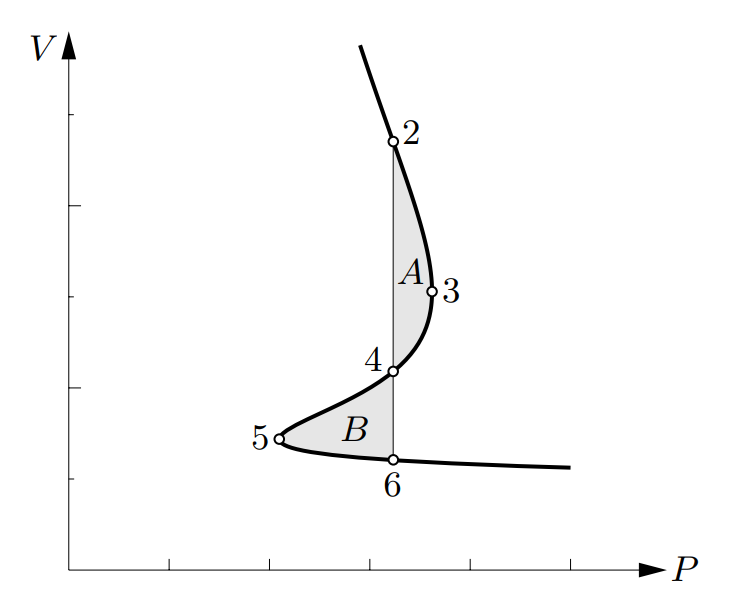
\includegraphics[width=0.4\linewidth]{images/fig3_9.png}
\end{figure}

\noindent
점 2에서 6까지 오름차순으로 삼각형 경로를 한 바퀴 돌면, \underline{깁스 자유 에너지의 전체 변화는 0}이다.
\begin{equation}
    0 = \oint_{\text{loop}} dG = \oint_{\text{loop}} \left( \frac{\partial G}{\partial P} \right)_T dP = \oint_{\text{loop}} V \, dP
\end{equation}
이는 곧 A와 B의 넓이차가 0임을 의미하기도 한다. 따라서, 상변화 압력은 $PV$ 곡선에서 enclosed area가 서로 같도록 하는 압력으로 결정되어야 성립한다.

\vspace{4mm}\noindent
\textbf{Maxwell Construction}

\begin{figure}[h]
    \centering
    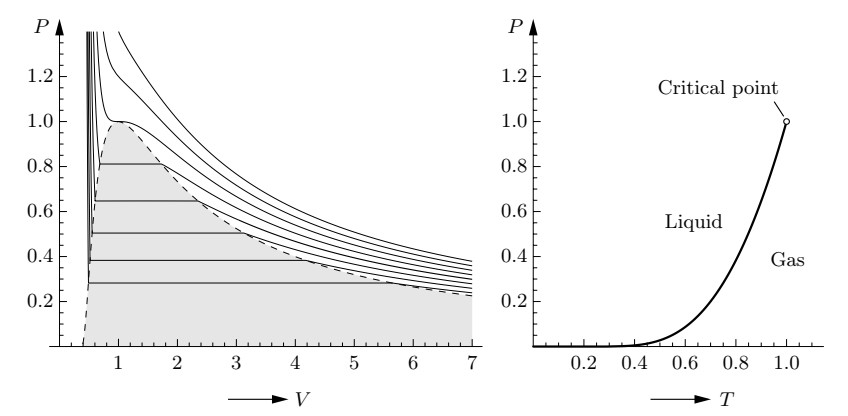
\includegraphics[width=0.75\linewidth]{images/fig3_10.png}
\end{figure}

\newpage

\section{Phase Transformation of Mixture}

아주 예전에 우리가 끓는점 배웠던걸 생각해보자. 물이랑 에탄올을 섞으면 78$^\circ$C에서 에탄올 한 번 날아가고, 100$^\circ$C에서 한 번 날아갔다. 그러나 혼합물은 그렇게 무 자르듯 두 온도에서 상변화가 일어나지 않았다. 따라서 순수 성분의 끓는점만 보고 혼합기체의 상전이를 예측하는 것은 부정확함. 그런고로, \underline{혼합물의 상평형 곡선}을 통해 해석하는 것이 바람직하다. 이번 절에선 혼합물의 상변화를 알아보자. 


\vspace{3mm}\noindent
\textbf{Gibbs Free Energy of a Mixture}

\begin{figure}[h]
    \centering
    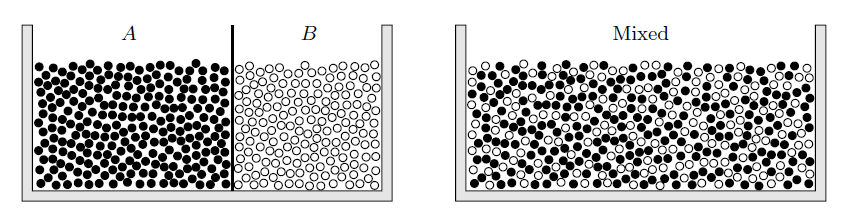
\includegraphics[width=0.75\linewidth]{images/fig4_1.png}
    \caption{두 종류의 분자가 섞이기 전후 모습이다.}
\end{figure}

첫 번째 근사로, 에너지나 부피의 변화는 무시하자. ($U$, $v$ fixed) 그러면 깁스 자유 에너지는 혼합 엔트로피에서 비롯할 것이다. 물질이 $x:1-x$로 존재하고 입자 총 개수는 $N$개임을 감안하자.
\begin{align}
    \Delta S_{\text{mixing}} &= k \ln [ {}_{N}C_{xN}] = k \ln \left[ \frac{N!}{(xN)! (N-xN)!} \right] \quad (\text{Strlling Approx.})\\
    &\approx k [ N \ln N - (xN) \ln(xN) - (N-xN) \ln (N-xN) ] \\
    &= -R[x\ln x + (1-x) \ln (1-x) ] \quad (\text{when }Nk \equiv R)
\end{align}
순수한 $A$와 $B$ 상태에서 1몰 당 깁스 자유에너지를 $G_A^\circ$, $G_B^\circ$라 하자. 깁스 자유 에너지에 대해선 다음이 성립한다.
\begin{align}
    G &= (1-x)G_A^\circ + xG_B^\circ  &(\text{No mixing})\\
    G &= (1-x)G_A^\circ + xG_B^\circ + \Delta S_{\text{mixing}} \cdot T &(\text{Ideal mixing})
\end{align}

\begin{figure}[h]
    \centering
    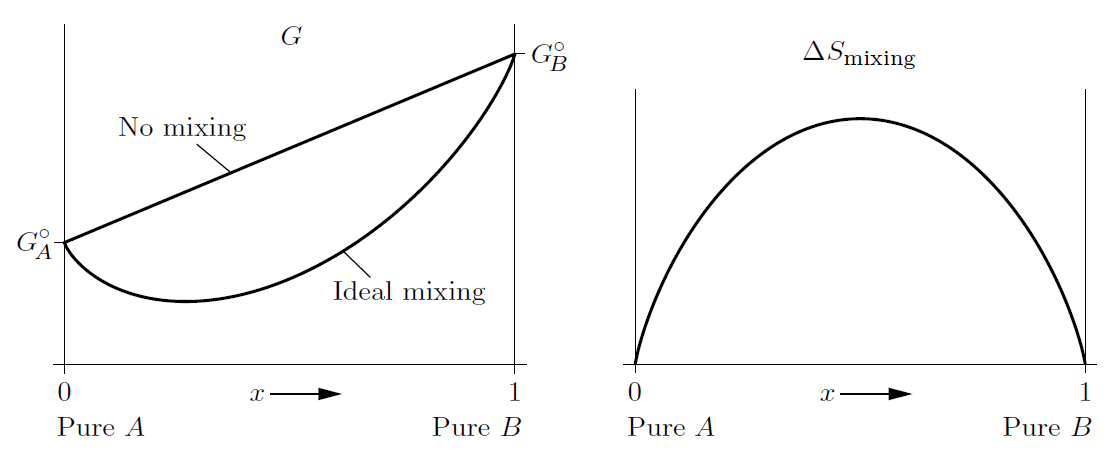
\includegraphics[width=0.7\linewidth]{images/fig4_2.png}
\end{figure}

유도한 바와 같이 simpie한 깁스 자유 에너지를 갖는 경우, \underline{ideal mixture}라고 한다. 실제로, $\Delta S_{\text{mixing}}$을 해석적으로 관찰할 경우, 다음과 같다.
\begin{equation}
    \frac{d}{dx} \Delta S_{\text{mixing}} \rightarrow \pm \infty \quad (\text{for }x \rightarrow 0, \ x \rightarrow 1)
\end{equation}
실제로, 구간의 endpoint들에선 기울기가 무한대로 발산해버리고, 이를 통해 \textcolor{blue}{equilibrium phase는 거의 항상 impurities를 갖고 있음}을 알수 있다. 만약, ideal하지 않게 섞이면 어떨까?

\newpage

\noindent
\textbf{Non-ideal Mixture}

만약, 혼합 과정에서 부피 변화를 무시할 때, $\Delta U_{\text{mixing}} \neq 0$이다!

\begin{figure}[h]
    \centering
    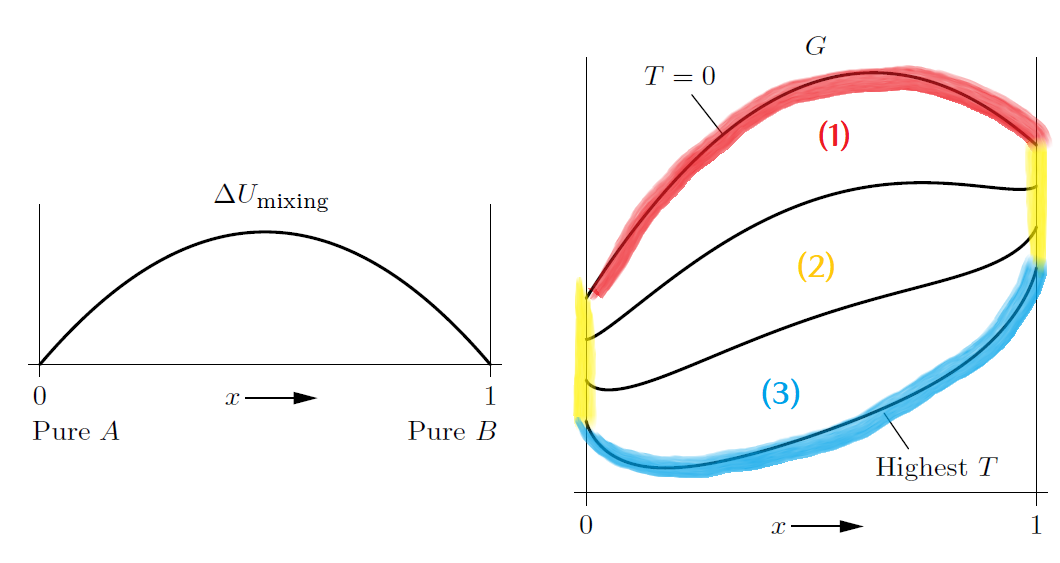
\includegraphics[width=0.7\linewidth]{images/fig4_3.png}
\end{figure}

\noindent
non-ideal한 상황에서, 깁스 자유 에너지는 다음과 같다.
\begin{equation}\label{eq:4-7}
    G = (1-x) G_A^\circ + xG_B^\circ + \color{blue} T \Delta S_{\text{mixing}} \color{black} + \color{red} \Delta U_{\text{mixing}} \color{black}
\end{equation}
(\ref{eq:4-7})은 위 그림의 3가지 경우에서 양상을 결정하는 항이 달라진다.
\begin{enumerate}
    \item[(1)] 구간에선 저온이고($T=0$), 이 땐, $U_{\text{mixing}}$이 dominate한다.
    \item[(2)] 와 같은 endpoint 근방에선 $\Delta S_{\text{mixing}}$이 dominate한다.
    \item[(3)] 구간에선 고온이고, 이 때 역시 $\Delta S_{\text{mixing}}$이 dominate한다.
\end{enumerate}

\begin{figure}[h]
    \centering
    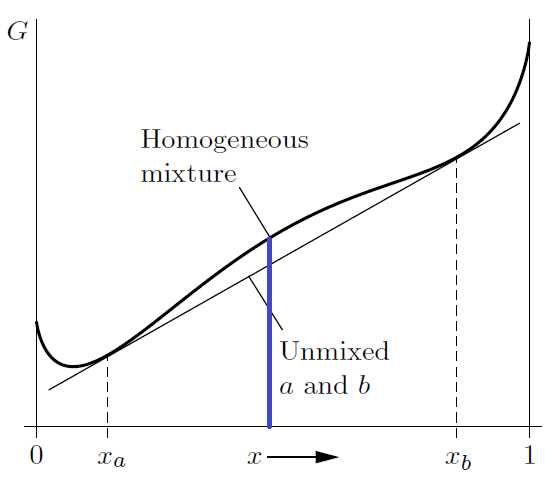
\includegraphics[width=0.4\linewidth]{images/fig4_4.png}
\end{figure}

위 깁스 자유에너지 그래프에서, 아래로 볼록한 두 구간의 양 끝에서 곡선에 접하는 가장 낮은 직선을 그려야 한다. 또한, 접선이 만나는 조성 구간 사이에서는, 혼합물이 자발적으로 $x_a$, $x_b$ 조성을 가진 두 상으로 분리된다. 그리고 특정 조성 $x$에 대해, 곡선에 접하는 직선이 가장 낮은 깁스 자유에너지 값을 준다.

우리는, $x_a$과 $x_b$ 사이 간격을 solubility gap이라 한다. 또한, 그 gap 안에 있는 상태를 immiscible하다 하고, 아닌 경우를 miscible하다고 한다. 아래 그림에서 왼쪽은 miscible, 오른쪽은 immiscible하다.

\begin{figure}[h]
    \centering
    
\includegraphics[width=0.75\linewidth]{images/fig4_5.png}
\end{figure}

\newpage

고체에서는, 두 물질을 혼합하면 보통 결정 격자에 큰 변형을 주어 에너지가 크게 증가하게 된다.

\begin{figure}[h]
    \centering
    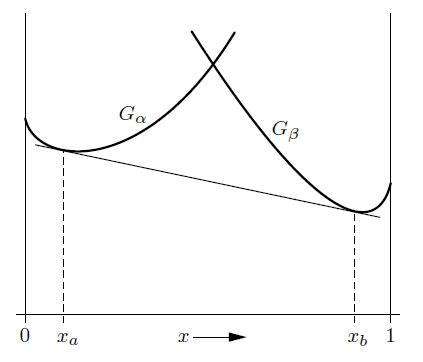
\includegraphics[width=0.4\linewidth]{images/fig4_7.png}
\end{figure}

\noindent
\textbf{Phase changes of a miscible mixture}

액체 질소와 액체 산소는 완전히 서로 섞일 수 있으므로, 액체 혼합물의 자유에너지 함수는 전체적으로 오목하다. 기체 혼합물의 자유에너지 역시 전체적으로 오목하다. 이 두 자유에너지 함수의 관계를 다양한 온도에서 비교해 보면, 시스템의 움직임과 phase diagram을 그릴 수 있다.

\begin{figure}[h]
    \centering
    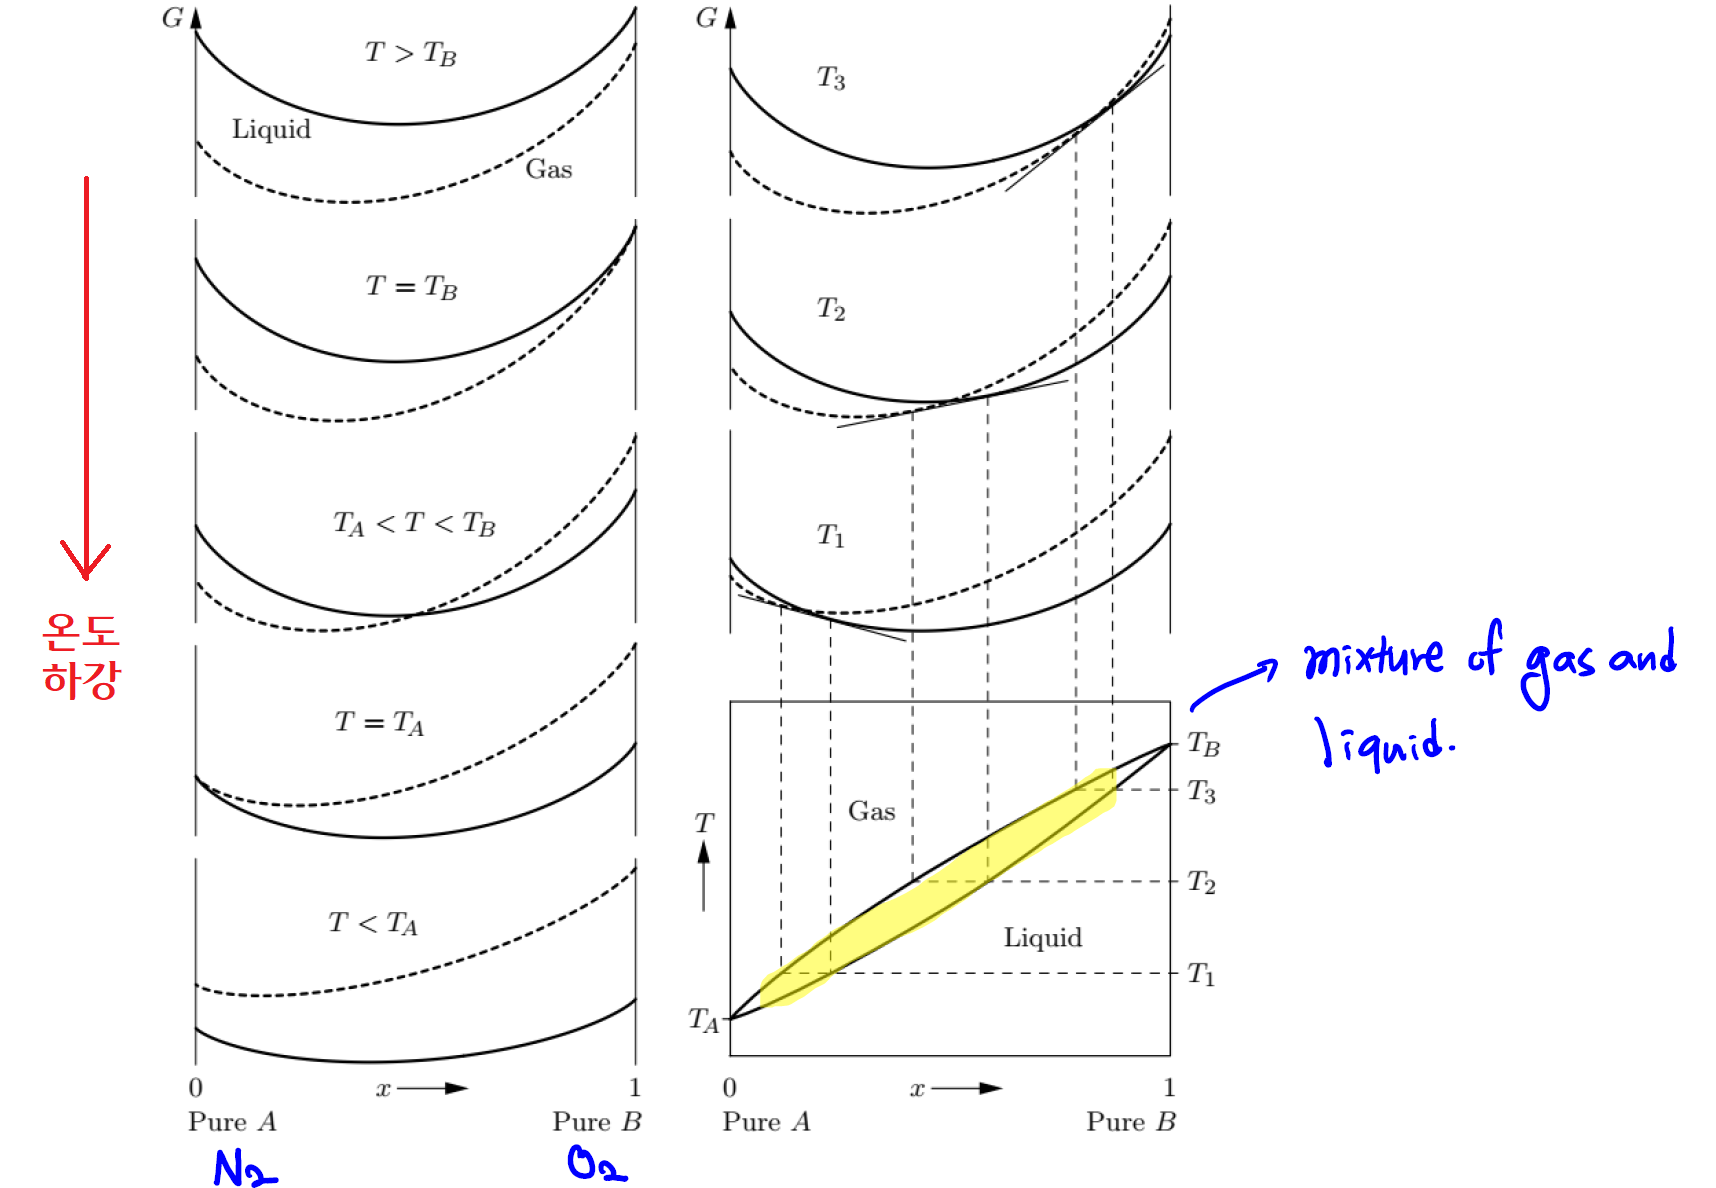
\includegraphics[width=0.9\linewidth]{images/fig4_8.png}
\end{figure}

엔트로피 $S>0$이고, 온도 $T$가 감소할 때, 다음의 identity를 떠올리자.
\begin{equation}
    \frac{\partial G}{\partial T} = -S
\end{equation}
이 경우, 깁스 자유 에너지는 증가한다. 또한, $S_{\text{gas}} > S_{\text{liquid}}$로부터, gas의 깁스 자유 에너지는 아주 빠르게 증가함.

\newpage

\begin{figure}[h]
    \centering
    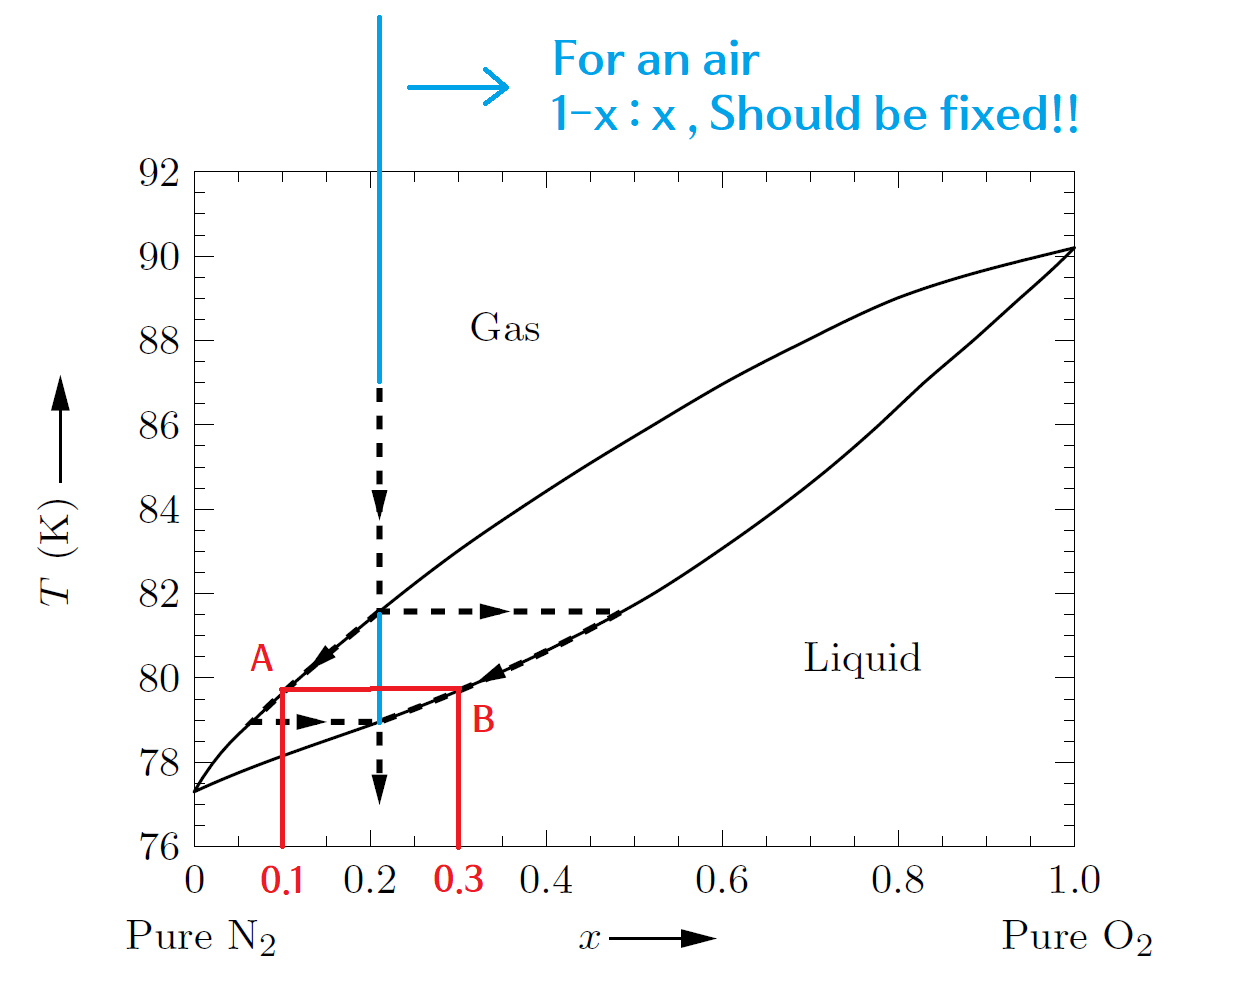
\includegraphics[width=0.67\linewidth]{images/fig4_9.png}
\end{figure}
\noindent
하늘색 점선의 경우, 대기의 조성비에 가깝도록 $x=0.21$정도로 설정한 선이다. 예를 들어, $T = 80$K에서, 는 기체와 액체 상태가 공존하는데, 기체의 경우 점 A처럼 산소 10\% + 질소 90\%로 존재하고, 액체는 점 B처럼 산소 30\%, 질소 70\%로 
혼합되어 존재한다. 또한, 양의 비율은 $A : B$로 주어진다.

\vspace{3mm}\noindent
\textbf{Phase changes of a eutectic system}

A와 B가 액체 상태에서는 완전히 섞일 수 있지만, 고체 상태에서는 서로 섞이지 않는 시스템의 고체–액체 상전이를 생각해보자. 이런 계의 이름을 공정계(eutectic system)라고 한다.

\begin{figure}[h]
    \centering
    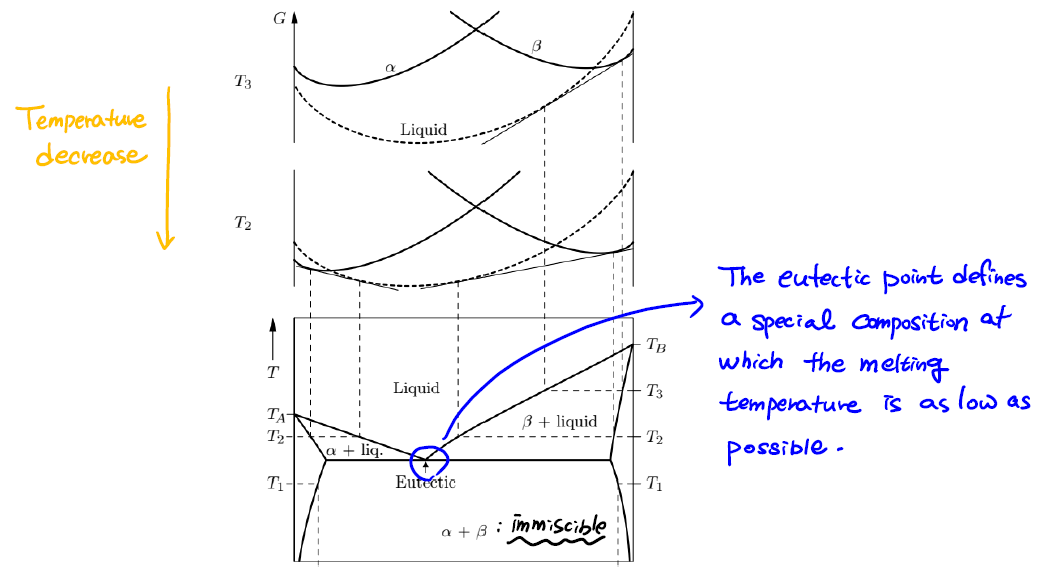
\includegraphics[width=1\linewidth]{images/fig4_10.png}
\end{figure}

공정점(eutectic point)은 녹는 온도가 가장 낮아지는 특별한 조성을 의미한다.

\newpage

\section{Dilute Solutions}

희석된 용액은 혼합물과 비슷하면서도, 용매를 주성분으로 본다는 점에서 차이가 있다. 용질 분자의 수가 용매 분자에 비해 훨씬 적을 때 용액이 희석(dilute)되었다고 한다. 

\begin{figure}[h]
    \centering
    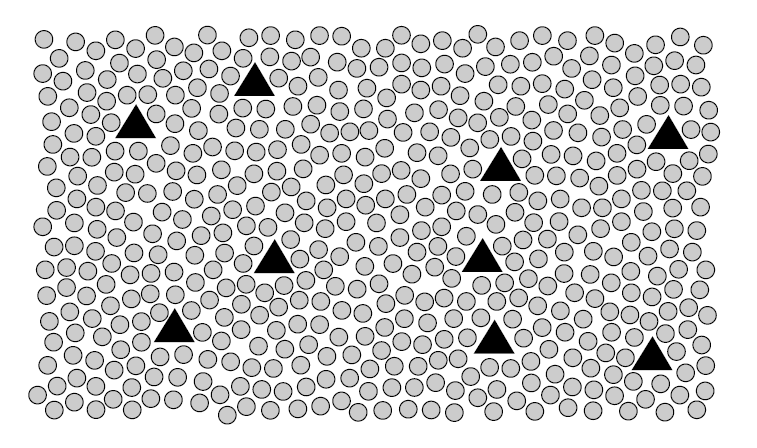
\includegraphics[width=0.4\linewidth]{images/fig5_1.png}
\end{figure}


순수한 용매에 대한 A 분자의 깁스 자유 에너지는 다음과 같다.
\begin{equation}
    G = N_A \mu_0 (T,P) \quad (\mu_0 \text{ is chem. potential in pure solvent})
\end{equation}
이제, 여기에 $B$ 분자를 더한다 가정하자. ($N_B \ll N_A$) 이 때, 온도와 압력은 고정한다.
\begin{equation}
    dG = dU + PdV - TdS = N_B = f(T,P) -TdS
\end{equation}
고정 조건들에 의해 $f(T,P)$가 생긴다. Mixing에 대한 엔트로피도 해석해보자.
\begin{align}
    dS = dS_{\text{mixing}} &= k \ln \binom{N_A + N_B}{N_B} = k \ln \frac{(N_A + N_B)!}{N_A ! N_B !}\\
    &\approx k [ (N_A + N_B) \ln (N_A + N_B) - N_A \ln N_A - N_B \ln N_B]\\
    &= k \left[ N_A \ln \left( \frac{N_A + N_B}{N_A} \right) + N_B \ln \left( \frac{N_A + N_B}{N_B} \right) \right]\\
    &\approx k \left[ N_A \cdot \frac{N_B}{N_A} + N_B \ln N_A - N_B \ln N_B \right]\\
    &= k [N_B + N_B \ln N_A - N_B \ln N_B]
\end{align}
따라서, mixing 깁스 자유에너지는 다음과 같다.
\begin{align}
    G_{\text{mixing}} &= N_A \mu_0 (T,P) + dG_{\text{mixing}}\\
    &= N_A \mu_0 (T,P) + N_B f(T,P) - N_B kT \ln N_A + N_B kT \ln N_B - N_B kT
\end{align}
따라서, 우리는 용매와 용질의 화학 퍼텐셜을 계산할 수 있다. $\mu_A$는 용매, $\mu_B$는 용질에 대한 값이다.
\begin{align}
    \mu_A &= \left( \frac{\partial G}{\partial N_A} \right)_{T,P,N_B} = \mu_0 (T,P) - \frac{N_B kT}{N_A}\\
    \mu_B &= \left( \frac{\partial G}{\partial N_B} \right)_{T,P,N_A} = f(T,P) + kT \ln (N_B / N_A)
\end{align}
용매의 화학 퍼텐셜에서, 용질이 많아질 수록 $\mu_A$는 감소한다. 또한, 용질의 화학 퍼텐셜은 다음 이상기체의 화학 퍼텐셜 공식과 유사하다.
\begin{equation}
    \mu_(T,P) = \mu^\circ (T) + kT \ln (P/P^\circ)
\end{equation}
다음으로 넘어가기 전, 농도에 대해 얘기하자면, 몰농도(molarity)는 \underline{용액 1L 당 용질의 몰수}, 몰랄농도(molality)는 \underline{용매 1kg 당 용질의 몰수}이다.

\newpage

따라서, 용액의 몰랄농도를 $m$이라 하자.\footnote{일반적으로 몰 농도는 $M$, 몰랄 농도는 $m$을 자주 사용한다.} 그러면 $\mu_B$는 다음과 같다.
\begin{equation}
    \mu_B = \left( \frac{\partial G}{\partial N_B} \right)_{T,P,N_A} = f(T,P) + kT \ln (N_B / N_A) = \mu_B^\circ (T,P) + kT \ln m_B
\end{equation}
여기서, $\mu_B^\circ (T,P)$는 용질 B의 몰랄 농도 $m=1$일 때의 화학 퍼텐셜이다.\footnote{표준 상태라고도 부른다.}

\vspace{3mm}\noindent
\textbf{Application of $\mu_A, \mu_B$ in solutions (Osmotic pressure)}

\begin{figure}[h]
    \centering
    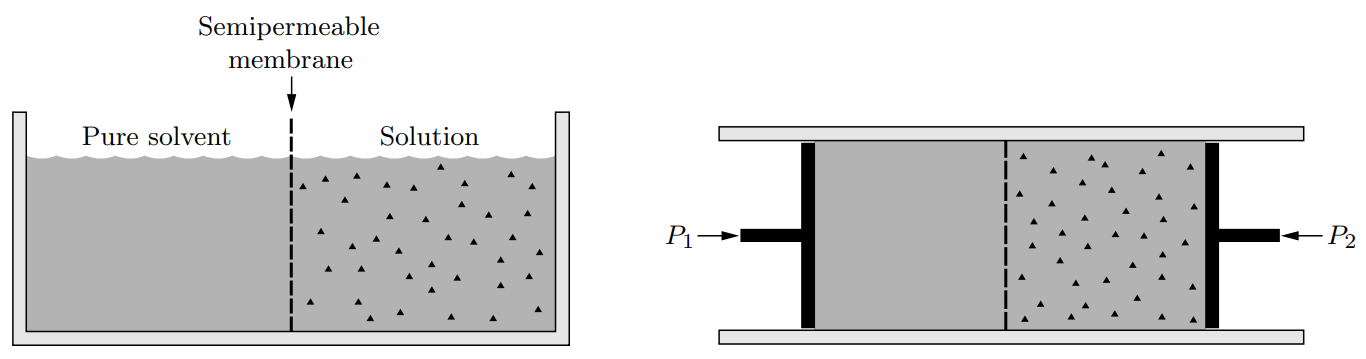
\includegraphics[width=0.9\linewidth]{images/fig5_2.png}
\end{figure}






\end{document}